\begin{frame}
	\myheading{Module 5.1: Learning Parameters : Infeasible (Guess Work)}
\end{frame}

\begin{frame}
	
	\begin{columns}
		
		\column{0.5\textwidth}
		\begin{overlayarea}{\textwidth}{\textheight}
			
\begin{tikzpicture}
	\node (input2) at (10,-0.1)  {$x_{1}$};
	\node [hidden_neuron] (neuron1) at (10,2)  {};
	\node (output0)  at (10,3.5) {$y$};
	\draw [->] (input2) -- (neuron1);
	\draw [->] (neuron1) -- (output0);
	\node (bias) at (8, 2) {$bias = w_0 = -0.5$};
	\node (weight) at (9.4,0.6) {$w_1 = 1$};
	\onslide<3->{\node (text) at (10,-0.7) {$criticsRating$};}
\end{tikzpicture}
			\only<4->{
				\vspace{-0.2in}
				\begin{figure}[!htp]
					\begin{center}
						\includegraphics<4-7>[scale=0.3]{images/module1/2sample_points.png}
						\includegraphics<8->[scale=0.3]{images/module1/2sample_points_sigmoid.png}
					\end{center}
				\end{figure}
			}
		\end{overlayarea}
		
		\column{0.5\textwidth}<2->
		\begin{overlayarea}{\textwidth}{\textheight}
			\only<2-3>{
				\begin{block}<2-3>{Input for training}
					$\{x_i, y_i\}^{N}_{i=1} \rightarrow N$ pairs of $(x,y)$
				\end{block}
				\begin{block}<3>{Training objective}
					Find $w$ and $b$ such that:\\
					$\displaystyle{\minimize_{w,b} \mathscr{L}(w,b) = \sum_{i=1}^{N} (y_i - f(x_i))^2}$
				\end{block}
			}
			
			\only<4->{
				\begin{block}{What does it mean to train the network?}
					\begin{itemize}\justifying
						\item<4-> Suppose we train the network with $ (x, y) = (0.5, 0.2)$ and $(2.5, 0.9)$  
						\item<5-> At the end of training we expect to find $w^*$, $b^*$ such that:
						\item<6-> $f(0.5) \rightarrow 0.2$ and  $f(2.5) \rightarrow 0.9$
					\end{itemize}
					
				\end{block}
				
				\begin{block}<7->{In other words...}
					\begin{itemize}\justifying
						\item We hope to find a sigmoid function such that $(0.5, 0.2)$ and $(2.5, 0.9)$ lie on this sigmoid
					\end{itemize}
				\end{block}
				
			}
		\end{overlayarea}
	\end{columns}
\end{frame}

%\subsection{Curve-fitting}
\begin{frame}
	\fontsize{16pt}{7.2}\selectfont
	\textit{Let us see this in more detail....}
\end{frame}

\begin{frame}
	\begin{columns}
		\column{0.35\textwidth}
		\begin{overlayarea}{\textwidth}{\textheight}
			\begin{onlyenv}<1->
				\begin{figure}[!htp]
					\begin{center}
						\includegraphics<1-2>[scale=0.3]{images/module1/2sample_points.png}
						\includegraphics<3-11>[scale=0.3]{images/module1/random/sig0.png}
						\includegraphics<12>[scale=0.3]{images/module1/random/sig1.png}
						\includegraphics<13>[scale=0.3]{images/module1/random/sig2.png}
						\includegraphics<14>[scale=0.3]{images/module1/random/sig3.png}
						\includegraphics<15>[scale=0.3]{images/module1/random/sig4.png}
						\includegraphics<16->[scale=0.3]{images/module1/random/sig5.png}
					\end{center}
				\end{figure}  
			\end{onlyenv}
		\end{overlayarea}
		
		\column{0.65\textwidth}
		\begin{overlayarea}{\textwidth}{\textheight}
			\only<2-5>{
				\begin{itemize}\justifying
					\item Can we try to find such a $w^*, b^*$ manually
					      \item<3-> Let us try a random guess.. (say, $w=0.5, b=0$)
					      \item<4-> Clearly not good, but how bad is it ?
					      \item<5-> Let us revisit $\mathscr{L}(w,b)$ to see how bad it is ... 
				\end{itemize}
			}
			
			\only<6-10>{
				\begin{align*}
					\onslide<6->{\mathscr{L}(w,b) & = \frac{1}{2} * \sum_{i=1}^{N} (y_i - f(x_i))^2}     \\
					\onslide<7->{                 & = \frac{1}{2} * ((y_1 - f(x_1))^2 + (y_2 - f(x_2))^2)} \\
					\onslide<8->{                 & = \frac{1}{2} * ((0.9 - f(2.5))^2 + (0.2 - f(0.5))^2)} \\
					\onslide<9->{                 & = 0.073}                                             
				\end{align*}
				\only<10->{\parbox[c][50pt][c]{230pt}{We want $\mathscr{L}(w,b)$ to be as close to 0 as possible}}
			}
			
			\only<11-> {
				Let us try some other values of $w$, $b$ 
				
				\begin{flushleft}
					\begin{table}
						\begin{tabular}{ccc}
							\hline
							\hline
							$w$               & $b$   & $\mathscr{L}(w,b)$ \\
							\hline
							\hline
							0.50              & 0.00  & 0.0730             \\
							\onslide<12-> {-0.10 & 0.00  & 0.1481}            \\
							\onslide<13-> {0.94  & -0.94 & 0.0214}            \\
							\onslide<14-> {1.42  & -1.73 & 0.0028}            \\
							\onslide<15-> {1.65  & -2.08 & 0.0003}            \\
							\onslide<16-> {1.78  & -2.27 & 0.0000}            \\
							\hline
							\hline
						\end{tabular}
					\end{table}
				\end{flushleft}
				
				\only<12>{\parbox[c][50pt][c]{230pt}{Oops!! this made things even worse...}}
				\only<13>{\parbox[c][50pt][c]{230pt}{Perhaps it would help to push w and b in the other direction...}}
				\only<14-15>{\parbox[c][50pt][c]{230pt}{Let us keep going in this direction, \textit{i.e.}, increase $w$ and decrease $b$}}
				\only<16>{\parbox[c][50pt][c]{230pt}{With some guess work and intuition we were able to find the right values for $w$ and $b$}}
			}
		\end{overlayarea}
	\end{columns}
	
\end{frame}

%\subsection{Error surfaces}
\begin{frame}
	\fontsize{16pt}{7.2}\selectfont
	\textit{Let us look at something better than our ``guess work'' algorithm....}
\end{frame}

\begin{frame}
	\begin{columns}
		\column{0.5\textwidth}
		\begin{overlayarea}{\textwidth}{\textheight}
			\begin{onlyenv}<1->
				\begin{figure}[!htp]
					\begin{center}
						\includegraphics<2->[scale=0.5]{images/module1/error_surface1.png}
					\end{center}
				\end{figure}  
			\end{onlyenv}
		\end{overlayarea}
		
		\column{0.5\textwidth}
		\begin{overlayarea}{\textwidth}{\textheight}
			\begin{itemize}\justifying
				\item Since we have only 2 points and 2 parameters ($w$, $b$) we can easily plot $\mathscr{L}(w,b)$ for different values of ($w$, $b$) and pick the one where $\mathscr{L}(w,b)$ is minimum
				      \item<3-> But of course this becomes intractable once you have many more data points and many more parameters !!
				      \item<4-> Further, even here we have plotted the error surface only for a small range of ($w$, $b$) [from $(-6, 6)$ and not from $(-\inf, \inf)$]
			\end{itemize}
		\end{overlayarea}
	\end{columns}
\end{frame}

\begin{frame}
	\fontsize{16pt}{7.2}\selectfont
	\textit{Let us look at the geometric interpretation of our ``guess work'' algorithm in terms of this error surface}
\end{frame}


\begin{frame}
	\begin{columns}
		\column{0.5\textwidth}
		\begin{overlayarea}{\textwidth}{\textheight}
			\begin{figure}[!htp]
				\begin{center}
					\only<1>{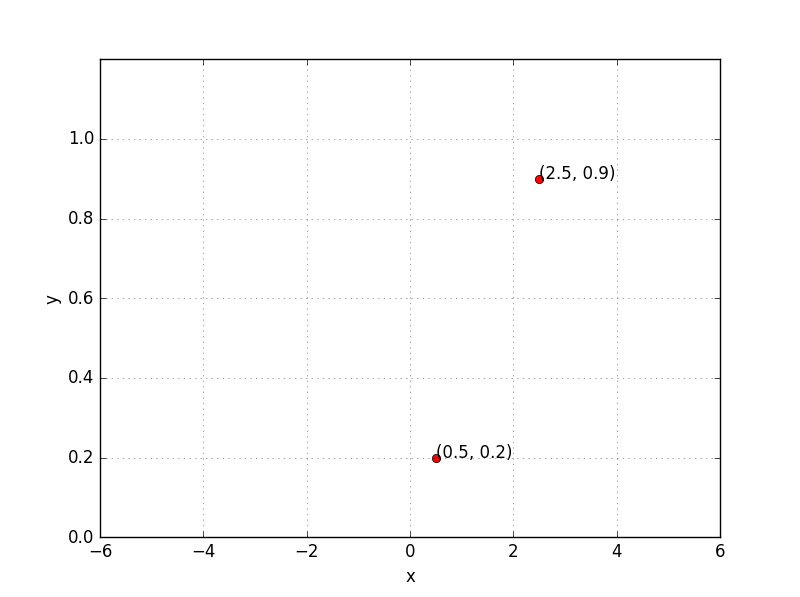
\includegraphics[width=1.0\textwidth]{images/module1/2sample_points.png}}
					\only<2>{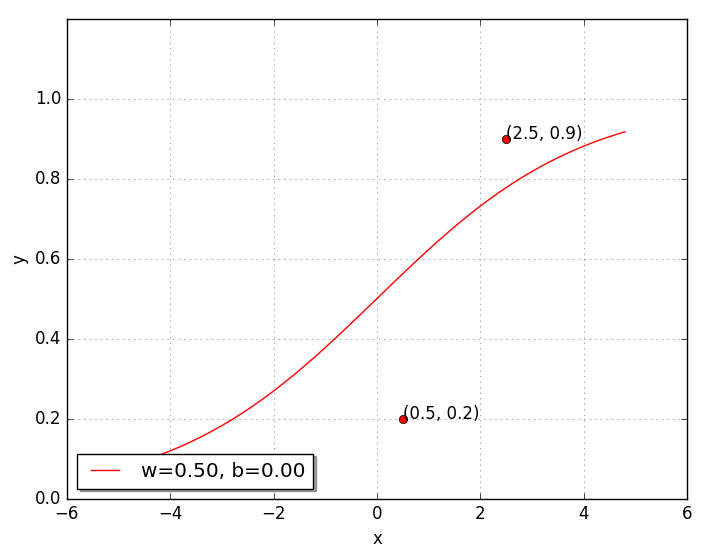
\includegraphics[width=1.0\textwidth]{images/module1/random/sig0.png}}
					\only<3>{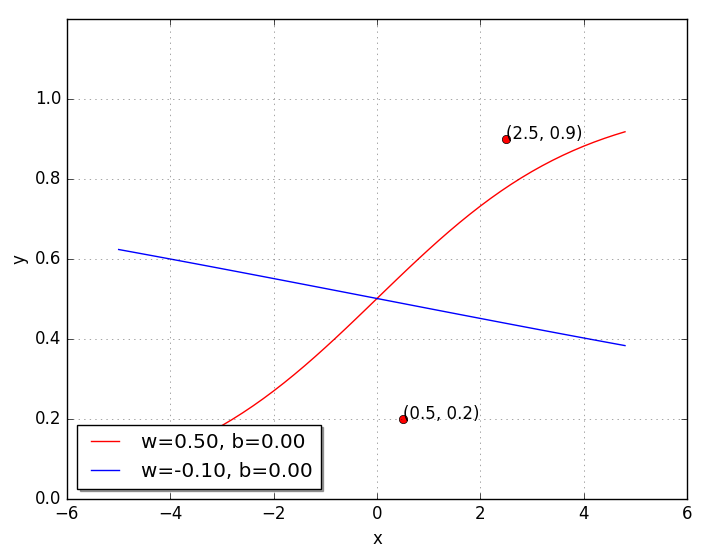
\includegraphics[width=1.0\textwidth]{images/module1/random/sig1.png}}
					\only<4>{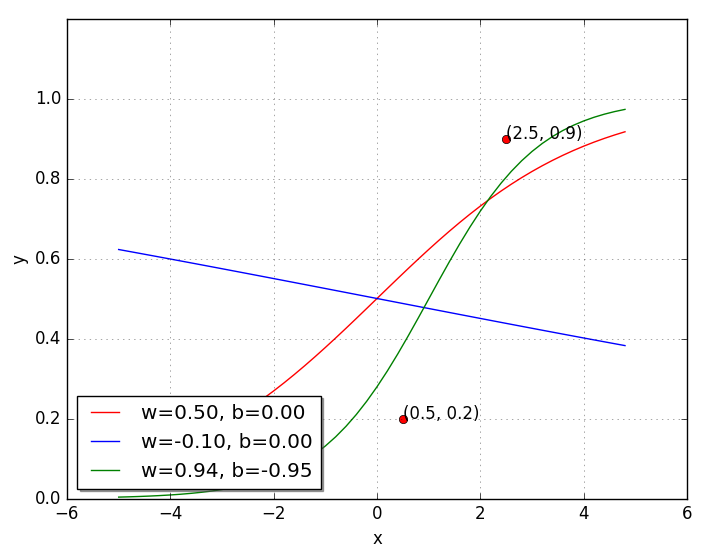
\includegraphics[width=1.0\textwidth]{images/module1/random/sig2.png}}
					\only<5>{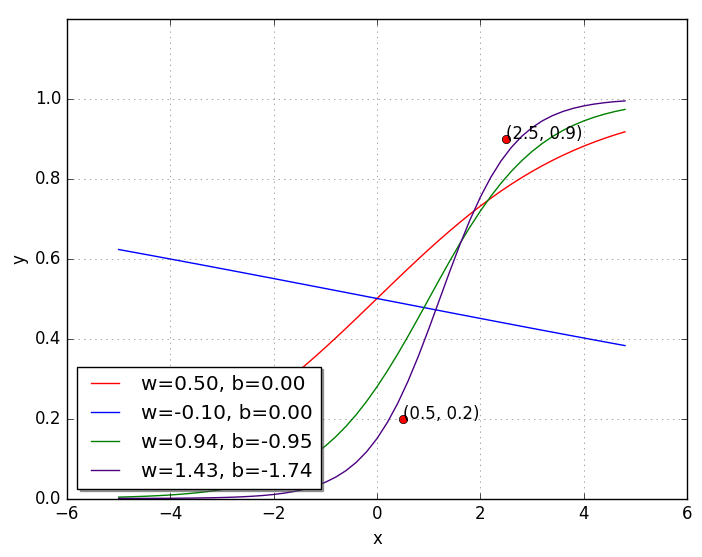
\includegraphics[width=1.0\textwidth]{images/module1/random/sig3.png}}
					\only<6>{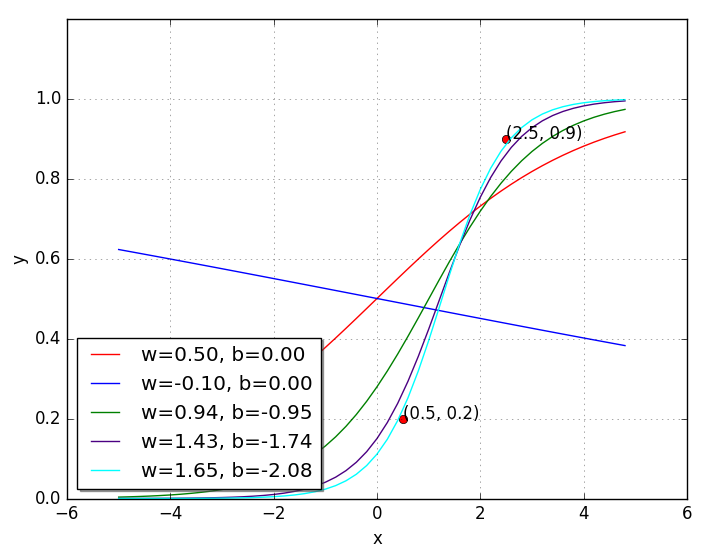
\includegraphics[width=1.0\textwidth]{images/module1/random/sig4.png}}
					\only<7->{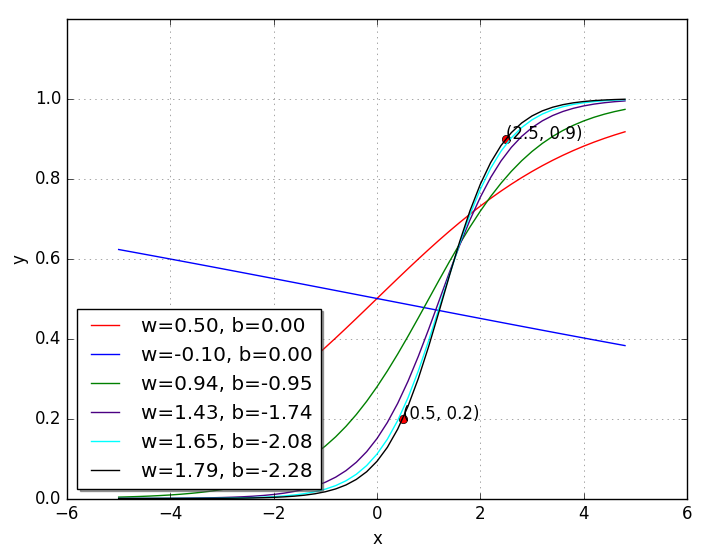
\includegraphics[width=1.0\textwidth]{images/module1/random/sig5.png}}
				\end{center}
			\end{figure}  
		\end{overlayarea}
		
		\column{0.5\textwidth}
		\begin{overlayarea}{\textwidth}{\textheight}
			\begin{figure}[!htp]
				\begin{center}
					\only<1>{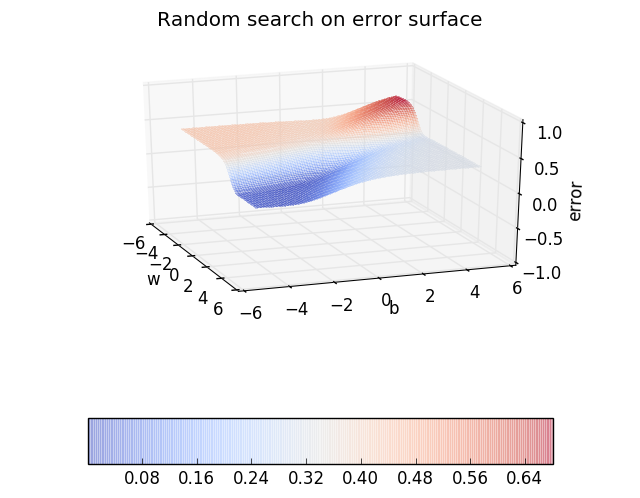
\includegraphics[width=1.0\linewidth]{images/module1/error_surface1.png}}
					\only<2>{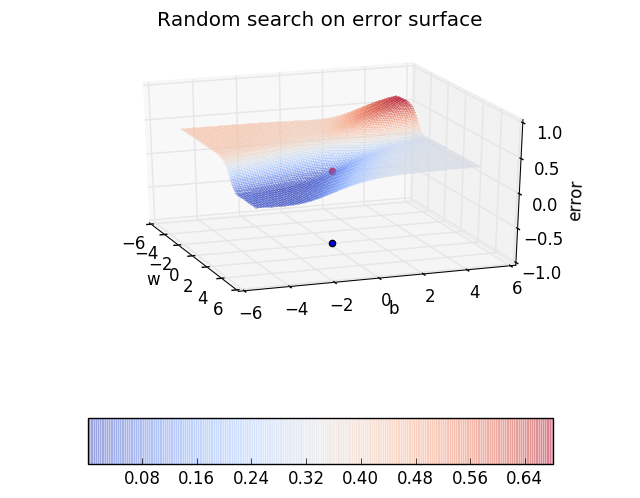
\includegraphics[width=1.0\linewidth]{images/module1/random/error0.png}}
					\only<3>{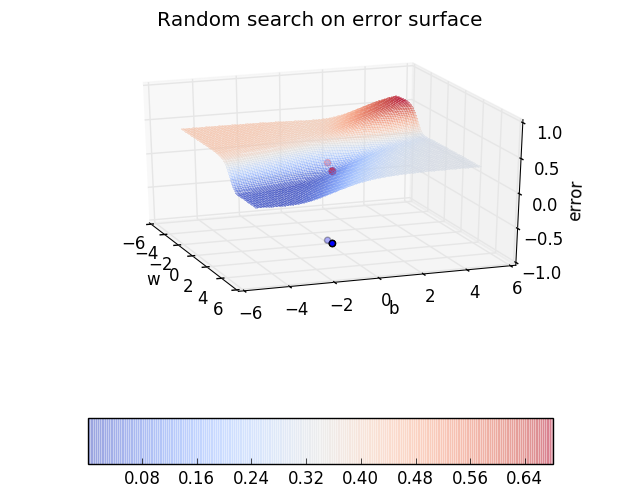
\includegraphics[width=1.0\linewidth]{images/module1/random/error1.png}}
					\only<4>{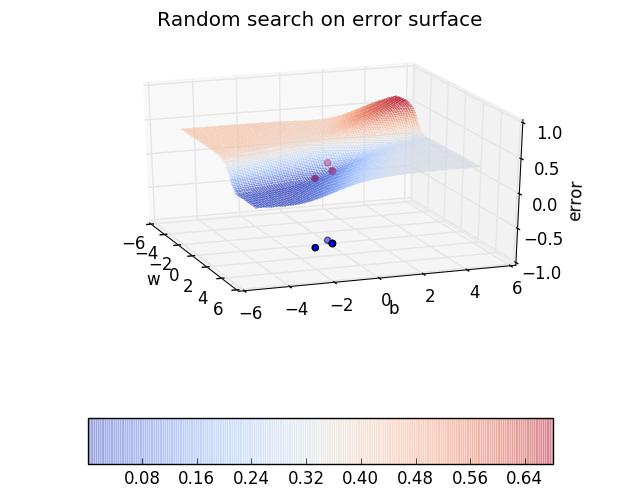
\includegraphics[width=1.0\linewidth]{images/module1/random/error2.png}}
					\only<5>{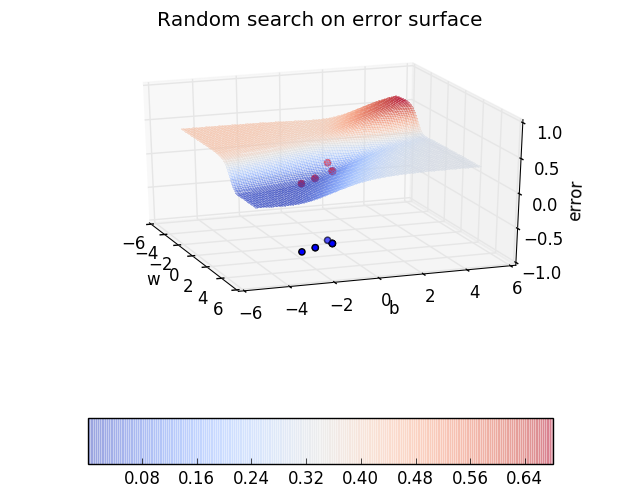
\includegraphics[width=1.0\linewidth]{images/module1/random/error3.png}}
					\only<6>{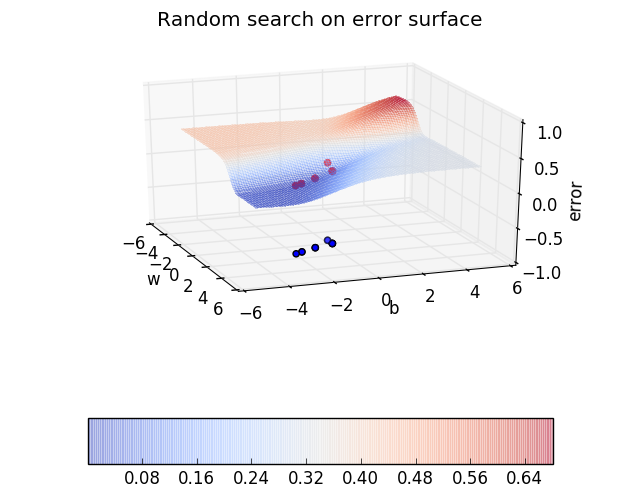
\includegraphics[width=1.0\linewidth]{images/module1/random/error4.png}}
					\only<7->{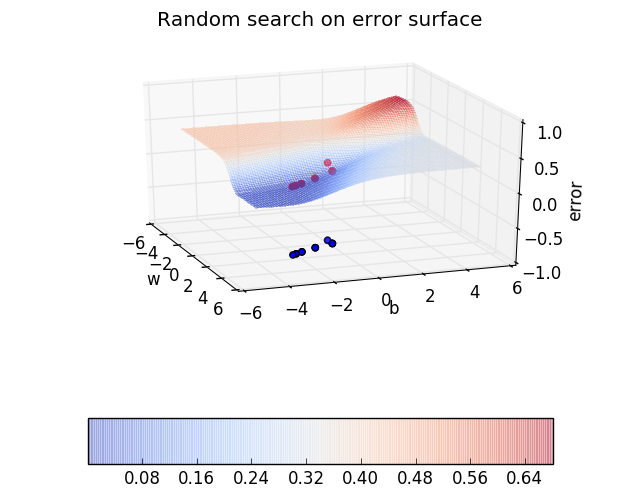
\includegraphics[width=1.0\linewidth]{images/module1/random/error5.png}}
				\end{center}
			\end{figure}  
		\end{overlayarea}
		
	\end{columns}
	
\end{frame}

